% This file was created by matlab2tikz.
%
%The latest updates can be retrieved from
%  http://www.mathworks.com/matlabcentral/fileexchange/22022-matlab2tikz-matlab2tikz
%where you can also make suggestions and rate matlab2tikz.
%
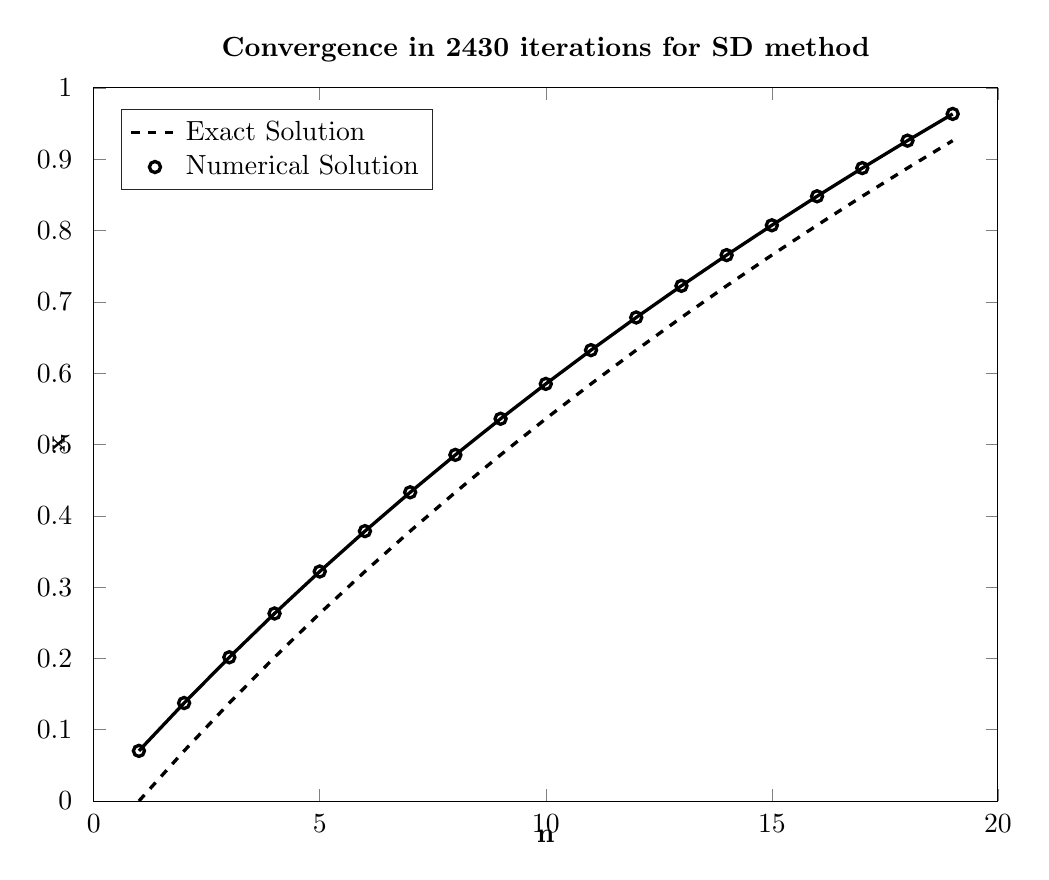
\begin{tikzpicture}

\begin{axis}[%
width=4.521in,
height=3.566in,
at={(0.758in,0.481in)},
scale only axis,
clip=false,
xmin=0,
xmax=20,
xtick={0,5,10,15,20},
xticklabels={\empty},
xlabel style={font=\bfseries},
xlabel={n},
ymin=0,
ymax=1,
ytick={0,0.1,0.2,0.3,0.4,0.5,0.6,0.7,0.8,0.9,1},
yticklabels={\empty},
ylabel style={font=\bfseries},
ylabel={x},
axis background/.style={fill=white},
title style={font=\bfseries},
title={Convergence in 2430 iterations for SD method},
legend style={at={(0.03,0.97)},anchor=north west,legend cell align=left,align=left,draw=white!15!black}
]
\addplot [color=black,dashed,line width=1.2pt]
  table[row sep=crcr]{%
1	0\\
2	0.070389327891398\\
3	0.137503523749935\\
4	0.20163386116965\\
5	0.263034405833794\\
6	0.321928094887362\\
7	0.37851162325373\\
8	0.432959407276106\\
9	0.485426827170242\\
10	0.53605290024021\\
11	0.584962500721156\\
12	0.632268215499513\\
13	0.678071905112638\\
14	0.722466024471091\\
15	0.765534746362977\\
16	0.807354922057604\\
17	0.84799690655495\\
18	0.887525270741587\\
19	0.925999418556223\\
};
\addlegendentry{Exact Solution};

\addplot [color=black,line width=1.2pt,only marks,mark=o,mark options={solid}]
  table[row sep=crcr]{%
1	0.070383296453508\\
2	0.137492951211586\\
3	0.201619954647232\\
4	0.263018149426247\\
5	0.321910295439018\\
6	0.378492945529996\\
7	0.432940401278212\\
8	0.485407949544979\\
9	0.536034531206194\\
10	0.584944957557161\\
11	0.632251763372296\\
12	0.67805676582851\\
13	0.722452383593942\\
14	0.765522759038333\\
15	0.807344717803179\\
16	0.847988593222949\\
17	0.887518937809073\\
18	0.925995139873374\\
19	0.963471960065584\\
};
\addlegendentry{Numerical Solution};

\addplot [color=black,solid,line width=1.2pt,forget plot]
  table[row sep=crcr]{%
1	0.070383296453508\\
2	0.137492951211586\\
3	0.201619954647232\\
4	0.263018149426247\\
5	0.321910295439018\\
6	0.378492945529996\\
7	0.432940401278212\\
8	0.485407949544979\\
9	0.536034531206194\\
10	0.584944957557161\\
11	0.632251763372296\\
12	0.67805676582851\\
13	0.722452383593942\\
14	0.765522759038333\\
15	0.807344717803179\\
16	0.847988593222949\\
17	0.887518937809073\\
18	0.925995139873374\\
19	0.963471960065584\\
};
\node[align=center, text=black]
at (axis cs:0,-0.031) {$0$};
\node[align=center, text=black]
at (axis cs:5,-0.031) {$5$};
\node[align=center, text=black]
at (axis cs:10,-0.031) {$10$};
\node[align=center, text=black]
at (axis cs:15,-0.031) {$15$};
\node[align=center, text=black]
at (axis cs:20,-0.031) {$20$};
\node[left, align=right, text=black]
at (axis cs:-0.258,0) {$0$};
\node[left, align=right, text=black]
at (axis cs:-0.258,0.1) {$0.1$};
\node[left, align=right, text=black]
at (axis cs:-0.258,0.2) {$0.2$};
\node[left, align=right, text=black]
at (axis cs:-0.258,0.3) {$0.3$};
\node[left, align=right, text=black]
at (axis cs:-0.258,0.4) {$0.4$};
\node[left, align=right, text=black]
at (axis cs:-0.258,0.5) {$0.5$};
\node[left, align=right, text=black]
at (axis cs:-0.258,0.6) {$0.6$};
\node[left, align=right, text=black]
at (axis cs:-0.258,0.7) {$0.7$};
\node[left, align=right, text=black]
at (axis cs:-0.258,0.8) {$0.8$};
\node[left, align=right, text=black]
at (axis cs:-0.258,0.9) {$0.9$};
\node[left, align=right, text=black]
at (axis cs:-0.258,1) {$1$};
\end{axis}
\end{tikzpicture}%